\documentclass[reqno,a4paper,12pt]{amsart}

\usepackage{amsmath,amssymb,amsthm,geometry,xcolor,soul,graphicx}
\usepackage{titlesec}
\usepackage{enumerate}
\usepackage{lipsum}
\usepackage{listings}
\RequirePackage[most]{tcolorbox}
\usepackage{braket}
%\usepackage{esint} %$\varoiint$ (带圈的二重积分)
%\usepackage[colorlinks,linkcolor=red]{hyperref} %\url{}超链接
\usepackage{xeCJK}
\setCJKmainfont{Kai}
\geometry{left=0.7in, right=0.7in, top=1in, bottom=1in}

\renewcommand{\baselinestretch}{1.3}

\title{固体物理第六次作业}
\author{董建宇 ~~ 2019511017}

\begin{document}

\maketitle
\titleformat{\section}[hang]{\small}{\thesection}{0.8em}{}{}
\titleformat{\subsection}[hang]{\small}{\thesubsection}{0.8em}{}{}

\section{(10.1) \textbf{Normal modes of a One-Dimensional Diatomic Chain} \\
(a) What is the difference between an acoustic mode and an optical mode. \\
$\triangleright$ Describe how particles move in each case. \\
(b) Derive the dispersion relation for the longitudinal oscillations if a one-dimensional diatomic mass-and-spring crystal where the unit cell is of length $a$ and each unit cell contains one atom of mass $m_1$ and one atom of mass $m_2$ connected together by springs with spring constant $\kappa$, as shown in the figure (all springs are the same, and motion of particles is in one dimension only). \\
\begin{centering}
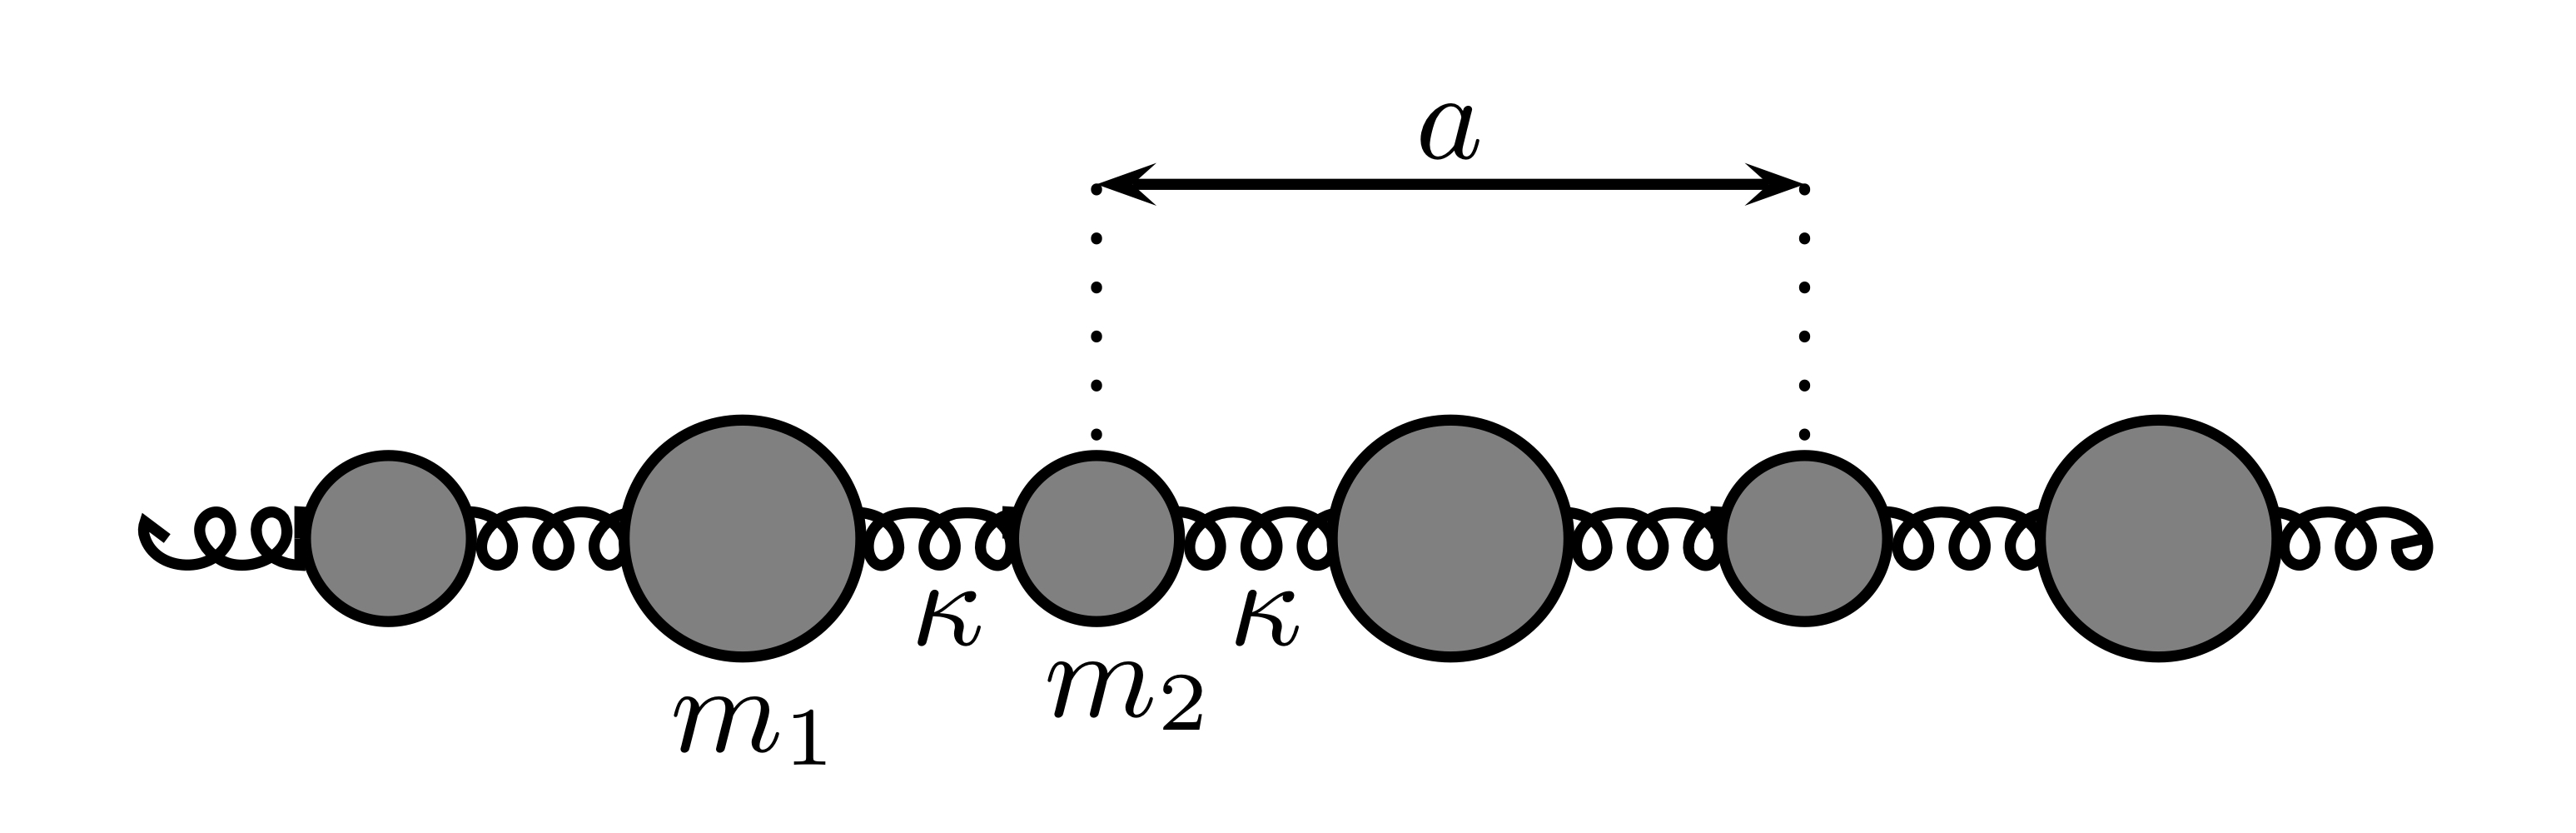
\includegraphics[scale=0.13]{10.1.jpeg}
\end{centering} \\
(c) Determine the frequencies of the acoustic and optical modes at $k=0$ as well as the Brillouin zone boundary \\
$\triangleright$ Describe the motion of the masses in each case (see margin note 4 of this chapter!) \\
$\triangleright$ Determine the sound velocity and show that the group velocity is zero at the zone boundary \\
(d) Sketch the dispersion in both reduced and extended zone scheme. \\
$\triangleright$ If there are $N$ unit cells, how many different normal modes are there? \\
$\triangleright$ How many $branches$ of excitations are there ? I.e., in reduced zone scheme, how many modes are there at each $k$? \\
(e) What happens when $m_1 = m_2$?
}

\begin{tcolorbox}[breakable, colback = black!5!white, colframe = black]
\begin{enumerate}[(a)]
\item For the acoustic mode, all atoms in the unit cell move in-phase with each other at $k = 0$, whereas for optical modes they move out of phase with each other at $k = 0$. Generally, an acoustic mode is any mode that has linear dispersion as $k \to 0$.\\
即对于声学模式,元胞中所有的原子在$k=0$时以同相位移动,对于光学模式,不同的原子在$k=0$时以不同的相位移动。

\item 考虑第$n$个质量为$m_1$的原子与第n个质量为$m_2$的原子,牛顿第二定律方程为:
\begin{align*}
	m_1\delta\ddot{x}_n = \kappa(\delta y_n - \delta x_n) + \kappa(\delta y_{n-1} - \delta x_n), \\
	m_2\delta\ddot{y}_n = \kappa(\delta x_{n+1} - \delta y_n) + \kappa(\delta x_n - \delta y_n).
\end{align*}
通解为:
\[
	\delta x_n = A_x e^{i(\omega t - kna)}, ~~ \delta y_n = A_y e^{i(\omega t - kna)}.
\]
代入方程可得:
\begin{align*}
	-m_1\omega^2A_x &= \kappa(1+e^{ika}) A_y - 2\kappa A_x, \\
	-m_2\omega^2A_y &= \kappa(1+e^{-ika}) A_x - 2\kappa A_y.
\end{align*}
关于$A_x$,$A_y$的方程组有非零解,则行列式为0:
\[
	\left\vert \begin{matrix}
		m_1\omega^2-2\kappa & \kappa(1+e^{ika}) \\
		\kappa(1+e^{-ika}) & m_2\omega^2-2\kappa
	\end{matrix}\right\vert = (m_1\omega^2 - 2\kappa)(m_2\omega^2 - 2\kappa) - 4\kappa^2\cos^2\frac{ka}{2} = 0.
\]
可以解得色散关系为:
\[
	\omega^2 = \frac{\kappa}{m_1m_2}(m_1+m_2 \pm \sqrt{m_1^2+m_2^2 + 2m_1m_2\cos(ka)}).
\]

\item 当$k=0$时,$\cos(ka) = 1$,则频率为:
\[
	\omega_- = 0, ~~ \omega_+ = \sqrt{\frac{2\kappa(m_1+m_2)}{m_1m_2}}.
\]
其中$\omega_-$为声学模式频率,$\omega_+$为光学模式频率。 \\
在布里渊区边界上时,有:$\cos(ka) = -1$,则频率为:
\[
	\omega_- = \sqrt{\frac{\kappa(m_1+m_2-\vert m_1-m_2\vert)}{m_1m_2}}, ~~ \omega_+ = \sqrt{\frac{\kappa(m_1+m_2+\vert m_1-m_2\vert)}{m_1m_2}}.
\]
其中$\omega_-$为声学模式频率,$\omega_+$为光学模式频率。 \\
\textcircled{1}当$k=0$,$\omega = \omega_- = 0$时,有$A_x = A_y$,即两种质量不同的原子以相同的频率,相同的振幅运动。 \\
\textcircled{2}当$k=0$,$\omega = \omega_+ = \sqrt{\frac{2\kappa (m_1+m_2)}{m_1m_2}}$时,有$A_x = -\frac{m_2}{m_1}A_y$,即两种质量不同的原子以相反的方向振动,质量更重的原子振幅较小。\\
当$\cos(ka) = -1$时,不妨令$m_1<m_2$,则有:$\omega_- = \sqrt{\frac{2\kappa}{m_2}}$, $\omega_+ = \sqrt{\frac{2\kappa}{m_1}}$. \\
\textcircled{3}当$\cos(ka) = -1$,$\omega = \omega_- = \sqrt{\frac{2\kappa}{m_2}}$时,有$A_x = 0$,最近邻两个质量为$m_2$的原子运动方向相反。 \\
\textcircled{4}当$\cos(ka) = -1$,$\omega = \omega_+ = \sqrt{\frac{2\kappa}{m_1}}$时,有$A_y = 0$,最近邻两个质量为$m_1$的原子运动方向相反。 \\
声速为:
\[
	v_{sound} = \lim_{k\to 0}\frac{d\omega_-}{dk} = \sqrt{\frac{a^2\kappa}{2(m_1+m_2)}}.
\]
由于群速度包涵$\sin(ka)$因子,则在布里渊区边界处有$v_{group} = 0$。 \\
原子链密度可以写为:$\rho = \frac{m_1+m_2}{a}$,压缩系数满足:$\frac{1}{\beta} = -L\frac{\partial F}{\partial L} = 2Na \frac{\kappa a/2}{2Na} = \frac{\kappa a}{2}$。则有:
\[
	\rho\beta = \frac{2(m_1+m_2)}{\kappa a^2} = v_{s}^{-2}.
\]

\item 令$m_2 = 2m_1 = 2m$, $x = ka$,则纵坐标为$\omega/\sqrt{\kappa/m}$。 \\
简约布里渊区中绘图如下:\\
\begin{centering}
	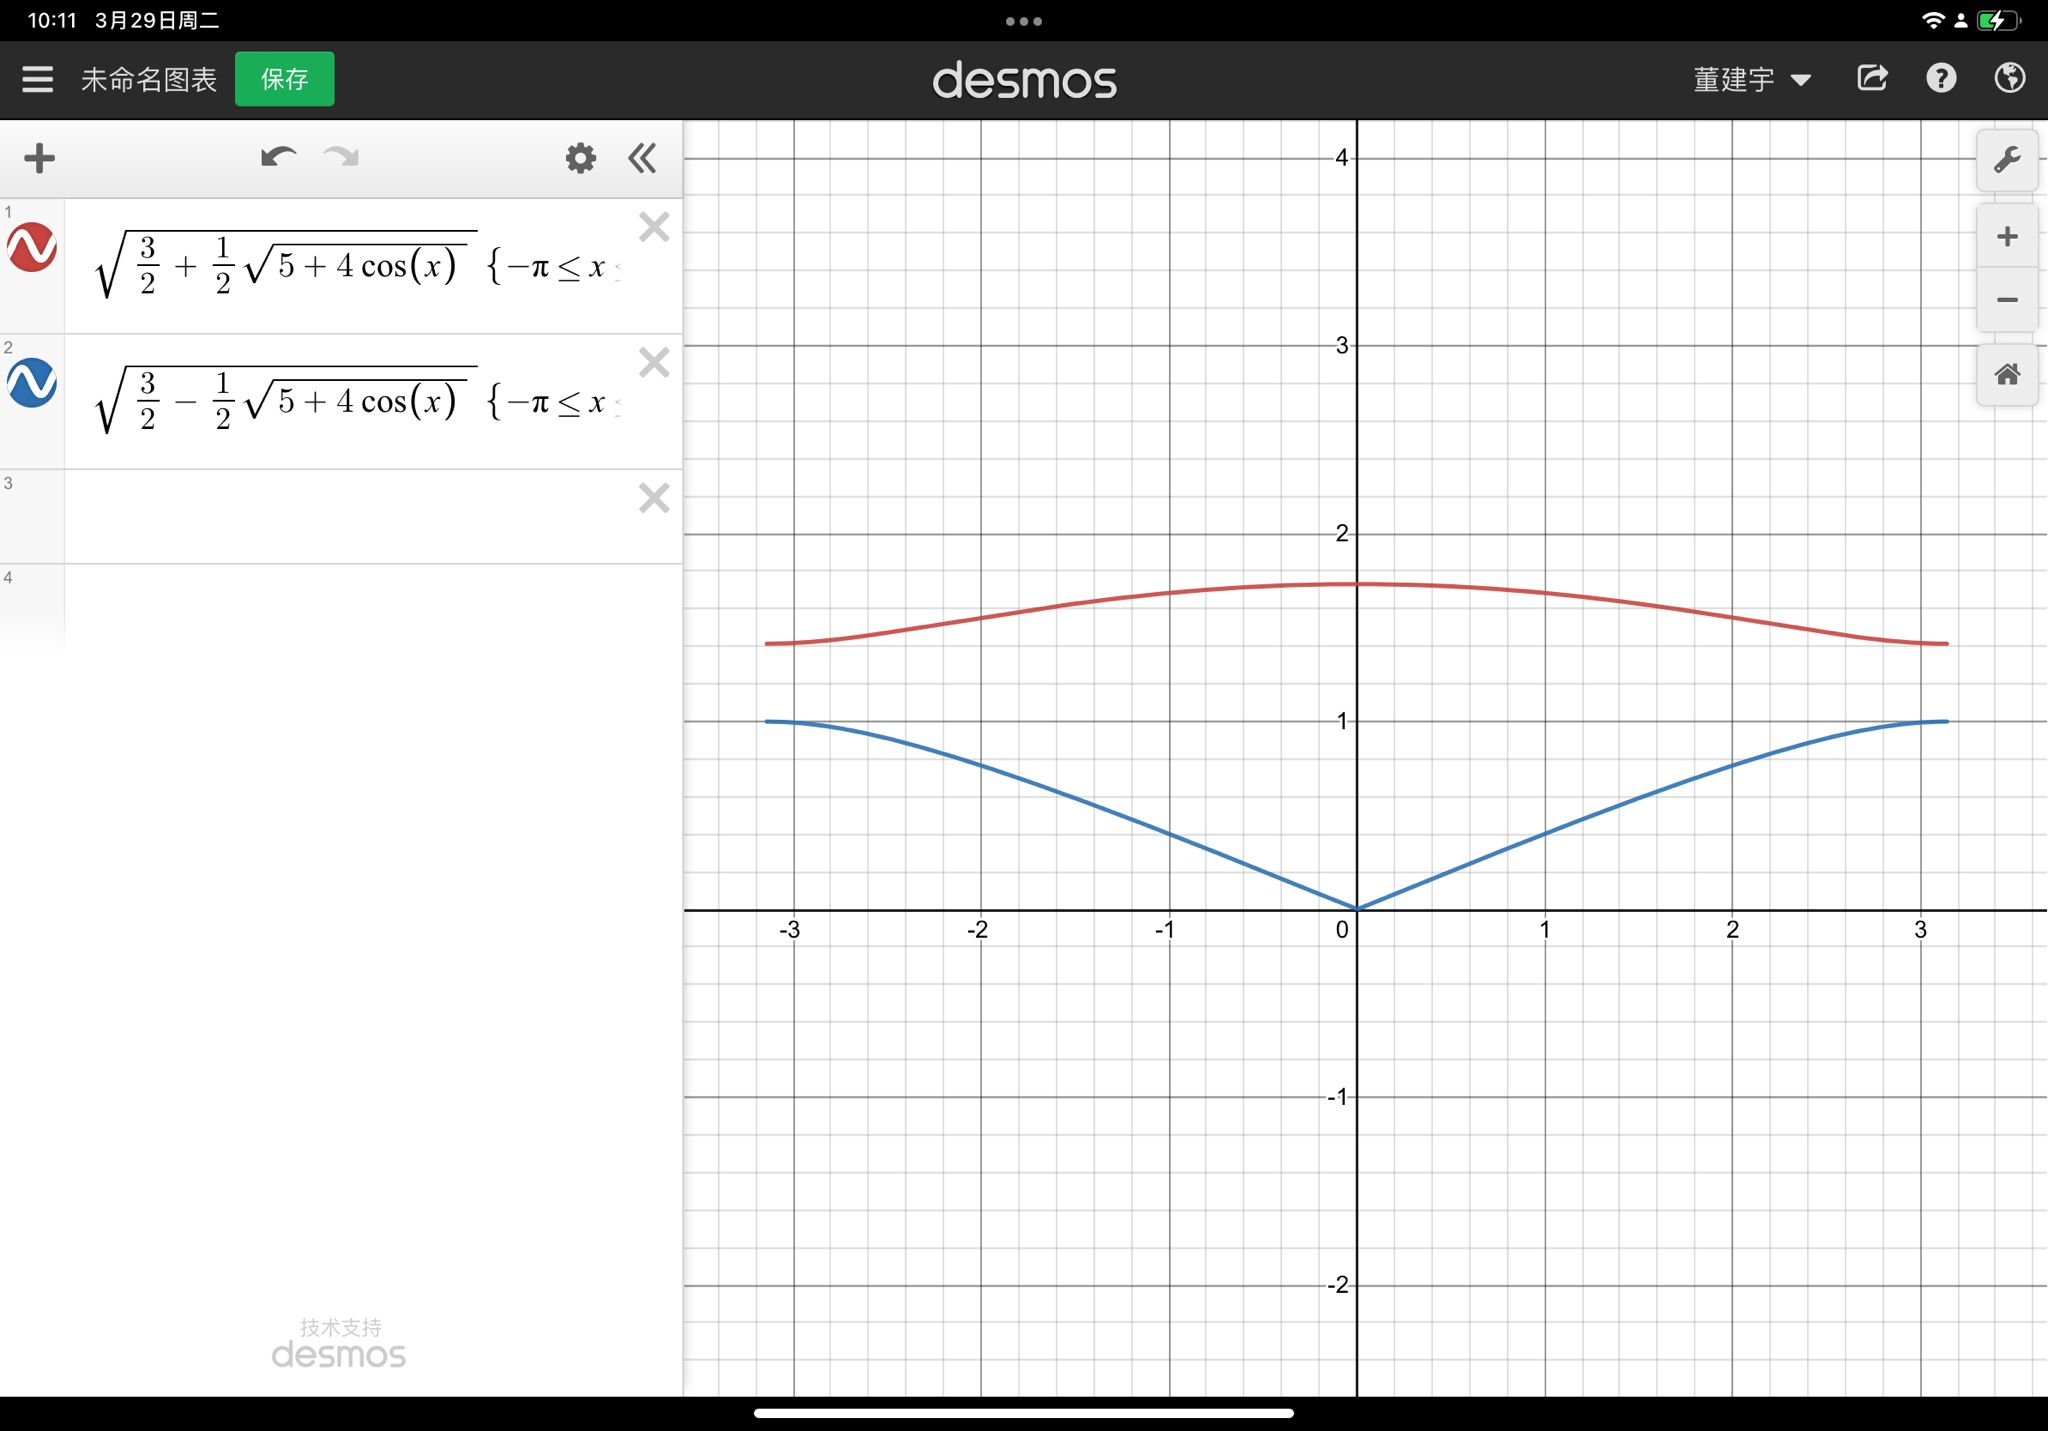
\includegraphics[scale=0.17]{reduced10.1.jpg}
\end{centering}\\
扩展布里渊区中绘图如下:\\
\begin{centering}
	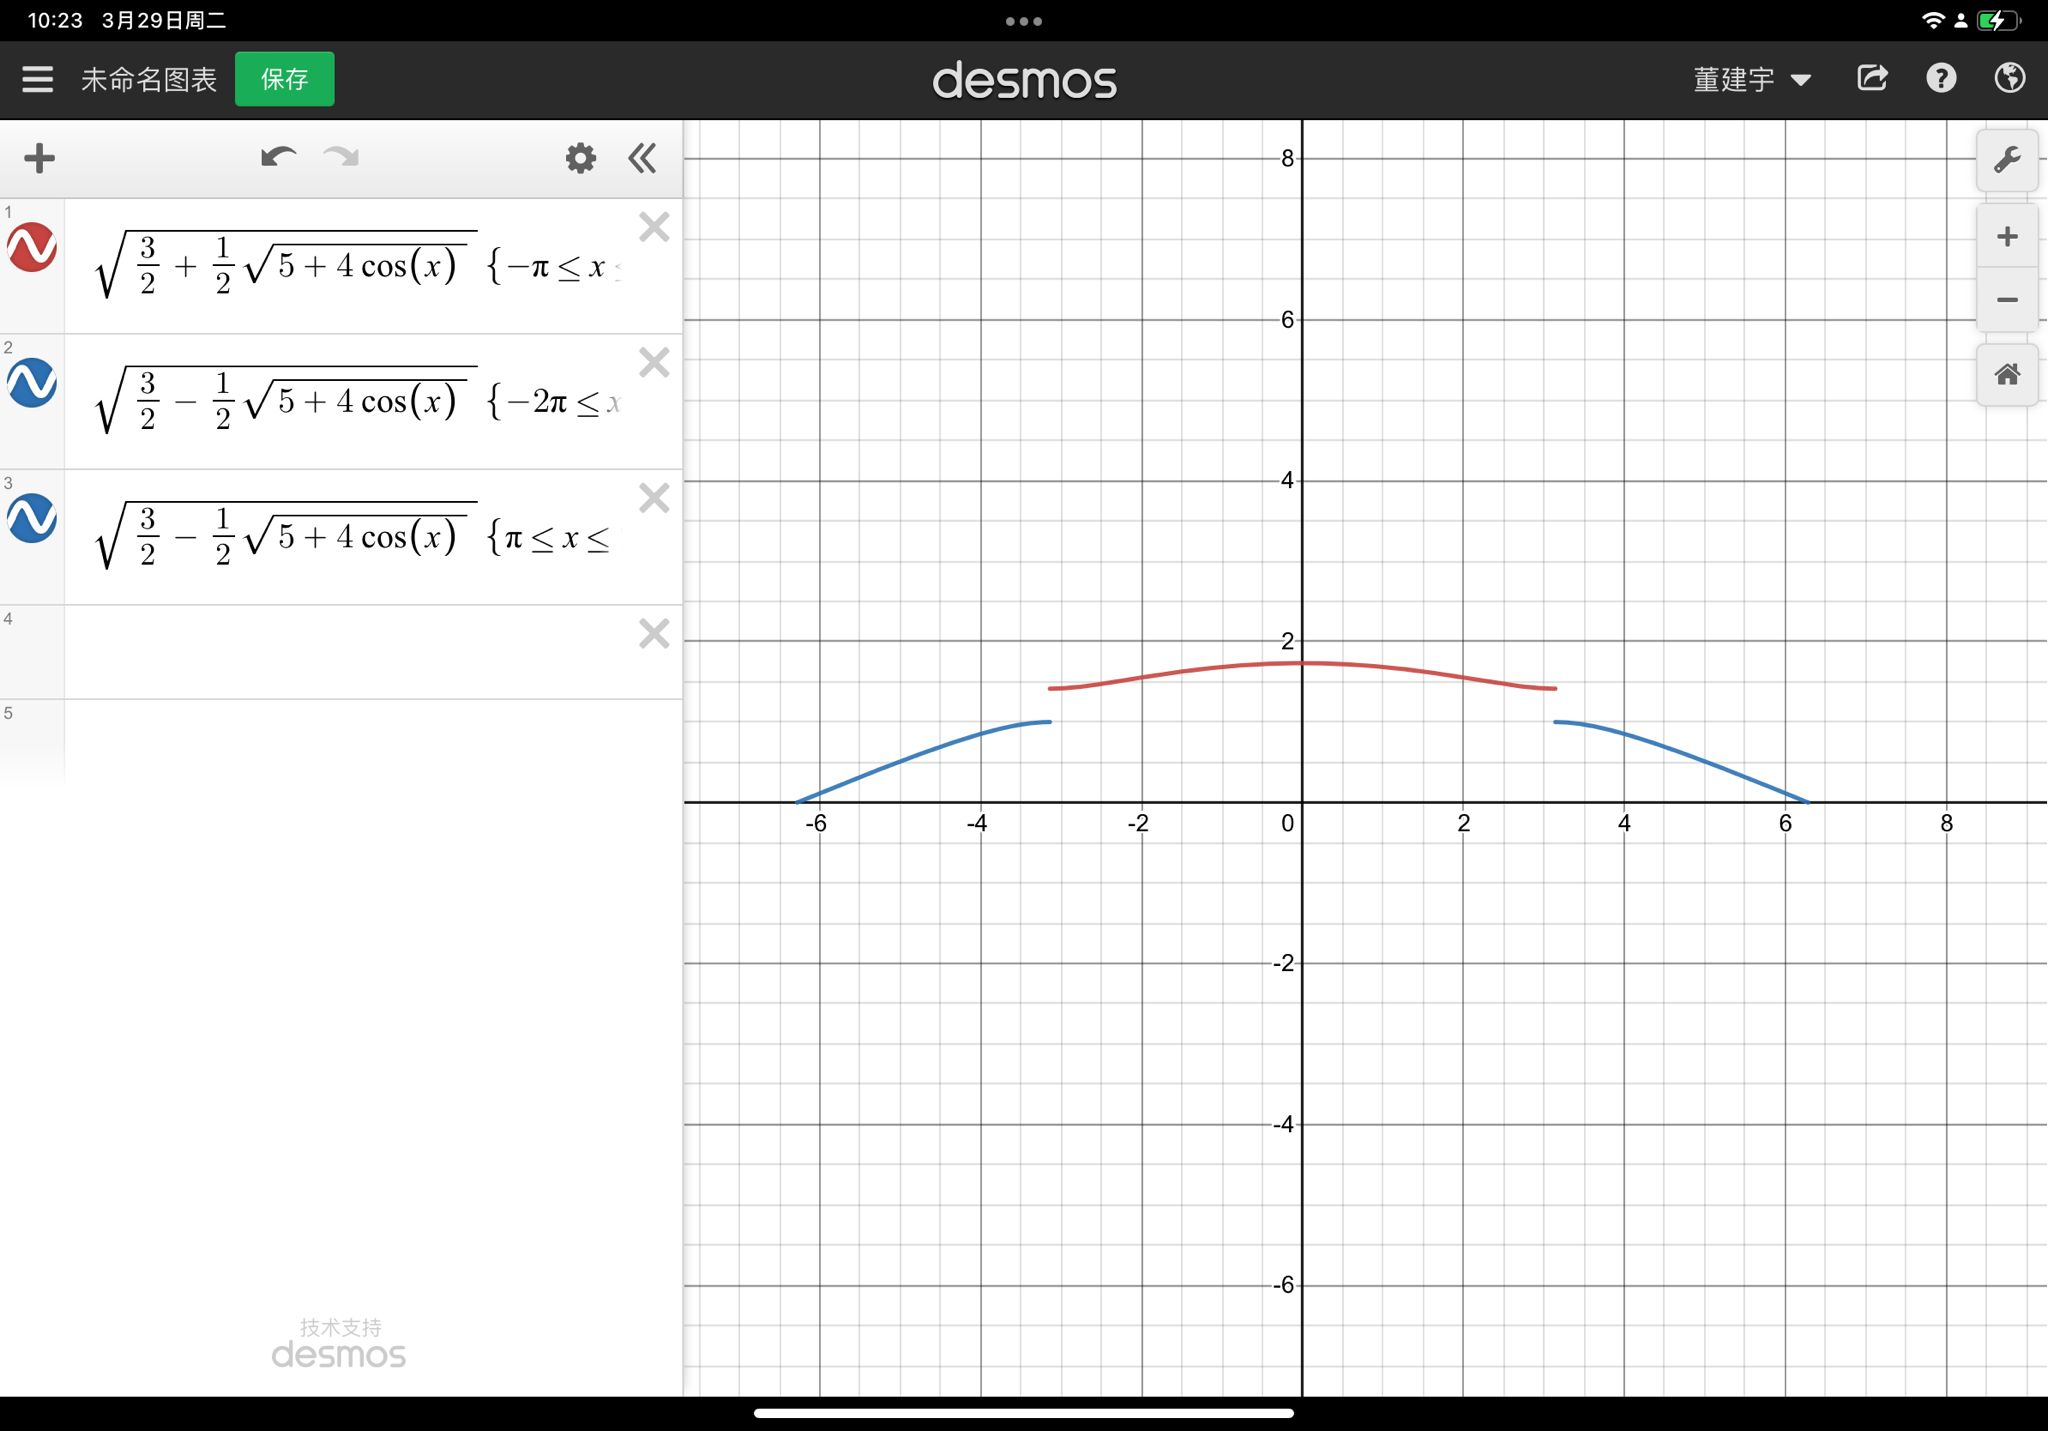
\includegraphics[scale=0.17]{extended10.1.jpg}
\end{centering}\\
如果有$N$个元胞,则有$2N$个原子,即有$2N$个简正模式。在reduced zone scheme 中,每一个$k$对应两个模式,即有$2$个分支。

\item 当$m_1 = m_2$时,系统变为相同原子的一位原子链,晶格常数变为$a/2$。布里渊区的宽度变为2倍。同时,布里渊区边界处的间隙消失,两个分支变为单个分支。
\end{enumerate}
\end{tcolorbox}


\section{\textbf{(10.5) Triatomic Chain} \\
Consider a mass-and-spring model with three different masses and three different springs per unit cell as shown in this diagram. \\
\begin{centering}
	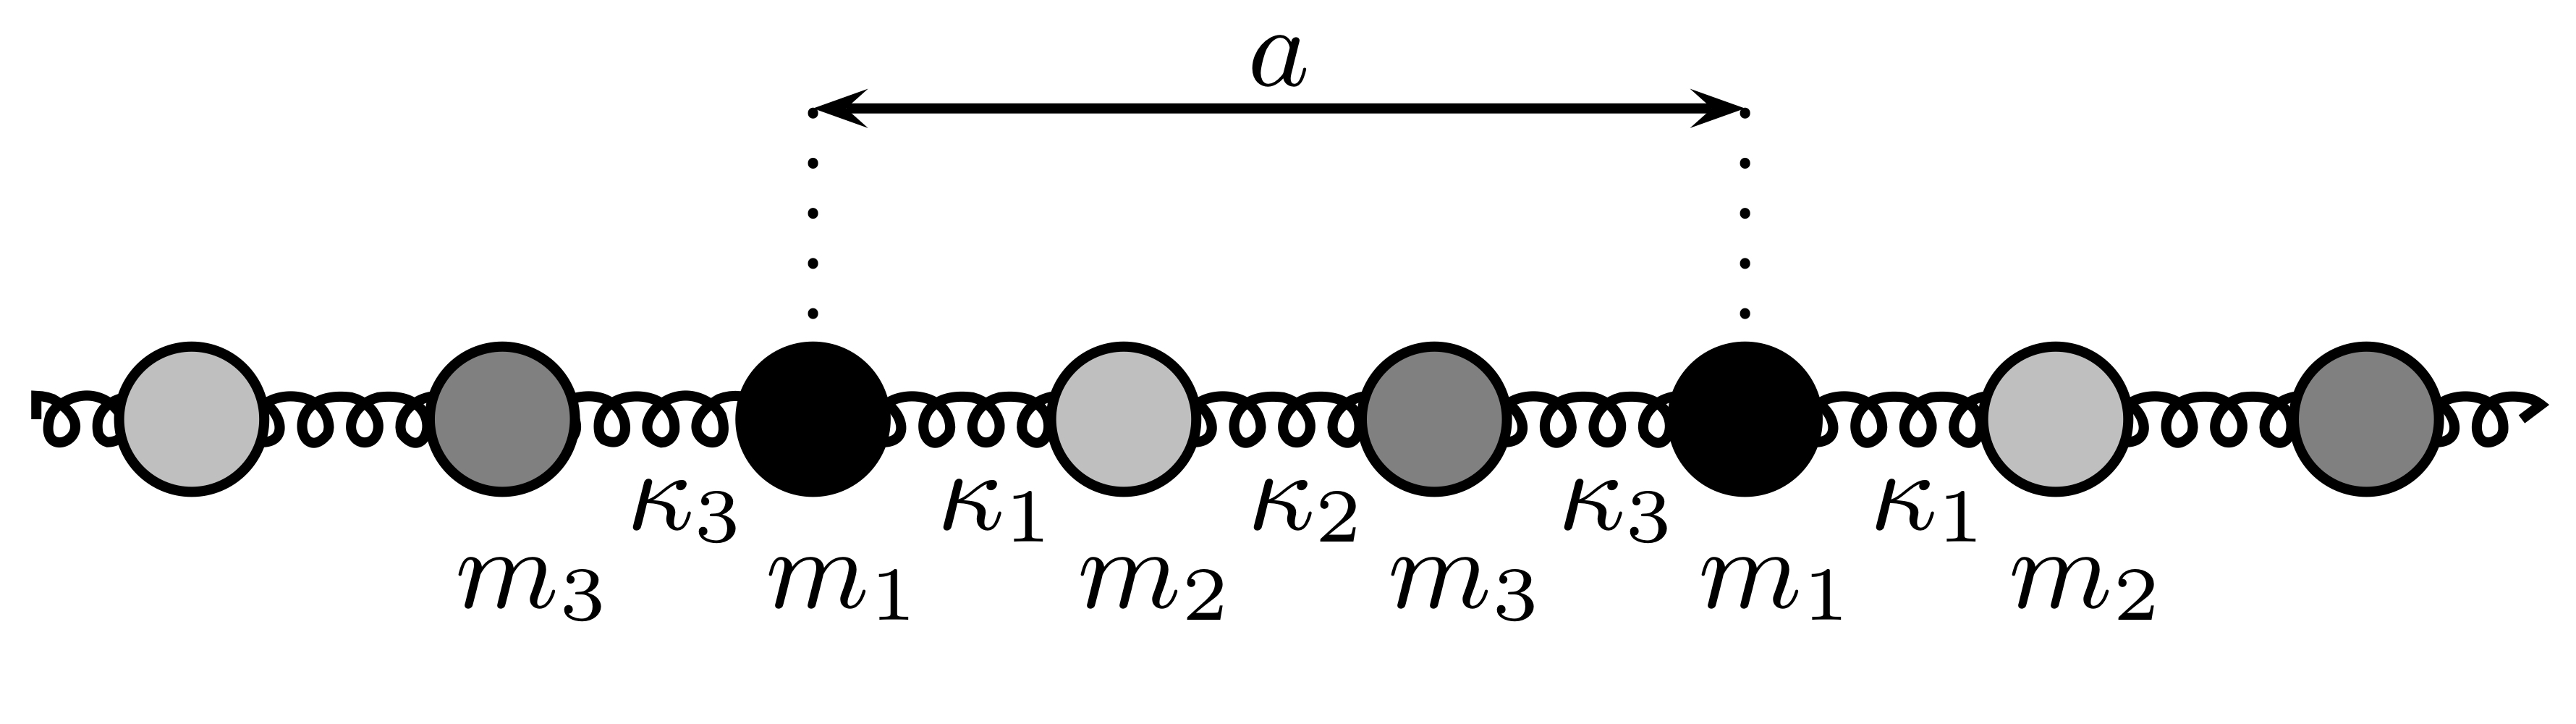
\includegraphics[scale = 0.13]{10.5.jpeg}
\end{centering} \\
As usual, assume that the masses move only in one dimension. \\
(a) At $k=0$ how many optical modes are there? Calculate the energies of these modes. Hind: you will get a cubic equation. However, you already know one of the roots since it is the energy of the acoustic mode at $k = 0$. \\
(b) If all the masses are the same and $\kappa_1 = \kappa_2$ determine the frequencies of all three modes at the zone boundary $k = \pi/a$. You will have a cubic equation, but you should be able to guess one root which corresponds to a particularly simple normal mode. \\
(c) If all three spring constants are the same, and $m_1 = m_2$ determine the frequencies of all three modes at the zone boundary $k=\pi/a$. Again you should be able to guess one of the roots.
}
\begin{tcolorbox}[breakable, colback = black!5!white, colframe = black]
\begin{enumerate}[(a)]
\item 当$k=0$时,有两个光学模式。考虑第$n$个元胞,由牛顿第二定律得:
\begin{align*}
	m_1\delta \ddot{x}_n &= \kappa_1(\delta y_n - \delta x_n) + \kappa_3(\delta z_{n-1} - \delta x_n), \\
	m_2\delta \ddot{y}_n &= \kappa_2(\delta z_n - \delta y_n) + \kappa_1(\delta x_n - \delta y_n), \\
	m_3\delta \ddot{z}_n &= \kappa_3(\delta x_{n+1} - \delta z_n) + \kappa_2(\delta y_n - \delta z_n).
\end{align*}
通解为:
\[
	\delta x_n = A_xe^{i(\omega t- kna)}, ~~ \delta y_n = A_ye^{i(\omega t- kna)}, ~~ \delta z_n = A_ze^{i(\omega t- kna)}.
\]
代入方程可得:
\begin{align*}
	&(\kappa_1+\kappa_3-m_1\omega^2)A_x - \kappa_1A_y - \kappa_3e^{ika}A_z = 0, \\
	&-\kappa_1 A_x + (\kappa_1+\kappa_2-m_2\omega^2)A_y - \kappa_2A_z = 0, \\
	&-\kappa_3 e^{-ika}A_x - \kappa_2A_y + (\kappa_2+\kappa_3-m_3\omega^2)A_z = 0.
\end{align*}
方程组存在非零解,则有:
\[
	\left\vert\begin{matrix}
		\kappa_1+\kappa_3-m_1\omega^2 & -\kappa_1 & -\kappa_3e^{ika} \\
		-\kappa_1 & \kappa_1+\kappa_2-m_2\omega^2 & -\kappa_2 \\
		-\kappa_3e^{-ika} & -\kappa_2 & \kappa_2+\kappa_3-m_3\omega^2
	\end{matrix}\right\vert = 0.
\]
即
\begin{align*}
	&-m_1m_2m_3\omega^6 + (m_1m_2(\kappa_2+\kappa_3) + m_1m_3(\kappa_1+\kappa_2) + m_2m_3(\kappa_1+\kappa_3))\omega^4 \\
	&- (m_1+m_2+m_3)(\kappa_1\kappa_2+\kappa_1\kappa_3+\kappa_2\kappa_3)\omega^2 + 2\kappa_1\kappa_2\kappa_3(1-\cos(ka)) = 0.
\end{align*}
当$k=0$时,有:
\[
	-\omega^6 + \left( \frac{\kappa_3+\kappa_1}{m_1} + \frac{\kappa_1+\kappa_2}{m_2} + \frac{\kappa_2+\kappa_3}{m_3} \right)\omega^4 - \frac{(m_1+m_2+m_3)(\kappa_1\kappa_2+\kappa_1\kappa_3+\kappa_2\kappa_3)}{m_1m_2m_3}\omega^2 = 0.
\]
易知对于声学模式有:
\[
	\omega_{acoustic} = 0
\]
则可以解得两个光学模式频率为:
\[
	\omega_{\pm} = \sqrt{\frac{1}{2}(\alpha \pm \sqrt{\alpha^2-4\beta})}.
	%\sqrt{\frac{1}{2}\left( \frac{\kappa_3+\kappa_1}{m_1} + \frac{\kappa_1+\kappa_2}{m_2} + \frac{\kappa_2+\kappa_3}{m_3} \right) \pm \sqrt{\left( \frac{\kappa_3+\kappa_1}{m_1} + \frac{\kappa_1+\kappa_2}{m_2} + \frac{\kappa_2+\kappa_3}{m_3} \right)^2 - \frac{4(m_1+m_2+m_3)(\kappa_1\kappa_2+\kappa_1\kappa_3+\kappa_2\kappa_3)}{m_1m_2m_3}}}.
\]
其中
\begin{align*}
	\alpha &= \frac{\kappa_3+\kappa_1}{m_1} + \frac{\kappa_1+\kappa_2}{m_2} + \frac{\kappa_2+\kappa_3}{m_3}, \\
	\beta &= \frac{4(m_1+m_2+m_3)(\kappa_1\kappa_2+\kappa_1\kappa_3+\kappa_2\kappa_3)}{m_1m_2m_3}.
\end{align*}
则能量为:
\[
	E_{\pm} = \hbar\omega_{\pm}.
\]

\item 如果质量全一样,且$\kappa_1 = \kappa_2$,频率满足的方程为:
\[
	m^3\omega^6 - m^2(4\kappa_1+2\kappa_3)\omega^4 + 3m(\kappa_1^2+2\kappa_1\kappa_3)\omega^2 - 4\kappa_1^2\kappa_3 = 0.
\]
注意到一种振动模式为与两个劲度系数$\kappa_1$连接的质量为$m_2$的原子保持不动,与劲度系数为$\kappa_3$连接的两个原子作为一个整体振动,且相邻两个元胞中与劲度系数$\kappa_3$连接的原子运动方向相反。则该振动频率为:
\[
	\omega_1^2 = \frac{\kappa_1}{m}.
\]
则有剩余两种频率满足:
\[
	\omega^4 - \frac{3\kappa_1+2\kappa_3}{m}\omega^2 + \frac{4\kappa_1\kappa_3}{m^2} = 0.
\]
则有:
\[
	\omega^2_{b,\pm} = \frac{3\kappa_1+2\kappa_2 \pm \sqrt{9\kappa_1^2 - 4\kappa_1\kappa_3 + 4\kappa_3^2}}{2m}.
\]

\item 如果劲度系数全一样,且$m_1=m_2$,频率满足的方程为:
\[
	m_1^2m_3\omega^6 - \kappa (4m_1m_3+2m_1^2) \omega^4 + 3\kappa^2(2m_1+m_3)\omega^2 - 4\kappa^2 = 0.
\]
注意到一种振动模式为质量为$m_3$的原子不动,质量相等的两个相邻原子作为一个整体,且相邻两个元胞中质量为$m_1$的原子振动方向相反。则该振动频率为:
\[
	\omega_1^2 = \frac{\kappa}{m_1}.
\]
则剩余两种频率满足:
\[
	\omega^4 - \frac{\kappa(2m_1+3m_3)}{m_1m_3}\omega^2 + \frac{4\kappa^2}{m_1m_3} = 0.
\]
则有:
\[
	\omega_{c,\pm}^2 = \frac{\kappa(2m_1+3m_3 \pm \sqrt{4m_1^2-4m_1m_3 + 9m_3^2})}{2m_1m_3}.
\]
\end{enumerate}
\end{tcolorbox}


\section{\textbf{(11.2) Diatomic Tight Binding Chain} \\
We now generalize the calculation of the previous exercise to a one-dimensional diatomic solid which might look as follows: 
\[
	-A-B-A-B-A-B-
\]
Suppose that the onsite energy of type $A$ is different from the onsite energy of type $B$. I.e., $\bra{n}H\ket{n}$ is $\epsilon_A$ for $n$ being on a site of type $A$ and is $\epsilon_B$ for $n$ being on a site of type $B$. (All hopping matrix elements $-t$ are still identical to each other.) \\
$\triangleright$ Calculate the new dispersion relation. (This is extremely similar to Exercise 10.1. If you are stuck, try studying that exercise again.) \\
$\triangleright$ Sketch this dispersion relation in both the reduced and extended zone schemes. \\
$\triangleright$ What happens if $\epsilon_A = \epsilon_B$? \\
$\triangleright$ What happens in the "atomic" limit when $t$ become very small. \\
$\triangleright$ What is the effective mass of an electron near the bottom of the lower band? \\
$\triangleright$ If each atom (of either type) is monovalent, is the system a metal or an insulator? \\
$\triangleright$ Given the results of this exercise, explain why LiF (which has very ionic bonds) is an extremely good insulator.
}
\begin{tcolorbox}[breakable, colback = black!5!white, colframe = black]
$\triangleright$ 记$\ket{n_A}$表示第n个元胞中原子A的态,$\ket{n_B}$表示第n个元胞中原子B的态,则系统态矢量为:
\[
	\ket{\Psi} = \sum_{n} (a_n\ket{n_A} + b_n\ket{n_B}).
\]
Hamiltonian为
\[
	H = \begin{pmatrix}
		\epsilon_A & -t & 0 & 0 & \cdots & 0 & -t \\
		-t & \epsilon_B & -t & 0 & \cdots & 0 & 0 \\
		0 & -t & \epsilon_A & -t & \cdots & 0 & 0 \\
		\vdots & \vdots & \vdots & \vdots & & \vdots & \vdots \\
		0 & 0 & 0 & 0 & \cdots & \epsilon_A & -t \\
		-t & 0 & 0 & 0 & \cdots & -t & \epsilon_B
	\end{pmatrix}.
\]
则有:
\begin{align*}
	Ea_n &= \epsilon_A a_n - t(b_n+b_{n-1}) \\
	Eb_n &= \epsilon_B b_n - t(a_n+a_{n+1})
\end{align*}
其中
\[
	a_n = Ae^{ikna}, ~~ b_n = Be^{ikna}.
\]
代入方程可得:
\begin{align*}
	&(\epsilon_A - E) A + t(1+e^{-ika})B = 0 \\
	&t(1+e^{ika}) A + (\epsilon_B - E) B = 0
\end{align*}
方程组存在非零解,则有:
\[
	\left\vert \begin{matrix}
		\epsilon_A - E & t(1+e^{-ika}) \\
		t(1+e^{ika}) & \epsilon_B - E 
	\end{matrix}\right\vert = E^2-(\epsilon_A+\epsilon_B)E + \epsilon_A\epsilon_B - 4t^2\cos^2(ka/2) = 0.
\]
可以解得:
\[
	E_{\pm} = \frac{1}{2}(\epsilon_A+\epsilon_B \pm \sqrt{(\epsilon_A-\epsilon_B)^2+16t^2\cos^2(ka/2)}).
\]
$\triangleright$ 选取$\epsilon_A = 2\epsilon_B = 2$, $t = \frac{1}{4}$,简约布里渊区绘图如下: \\
\begin{centering}
	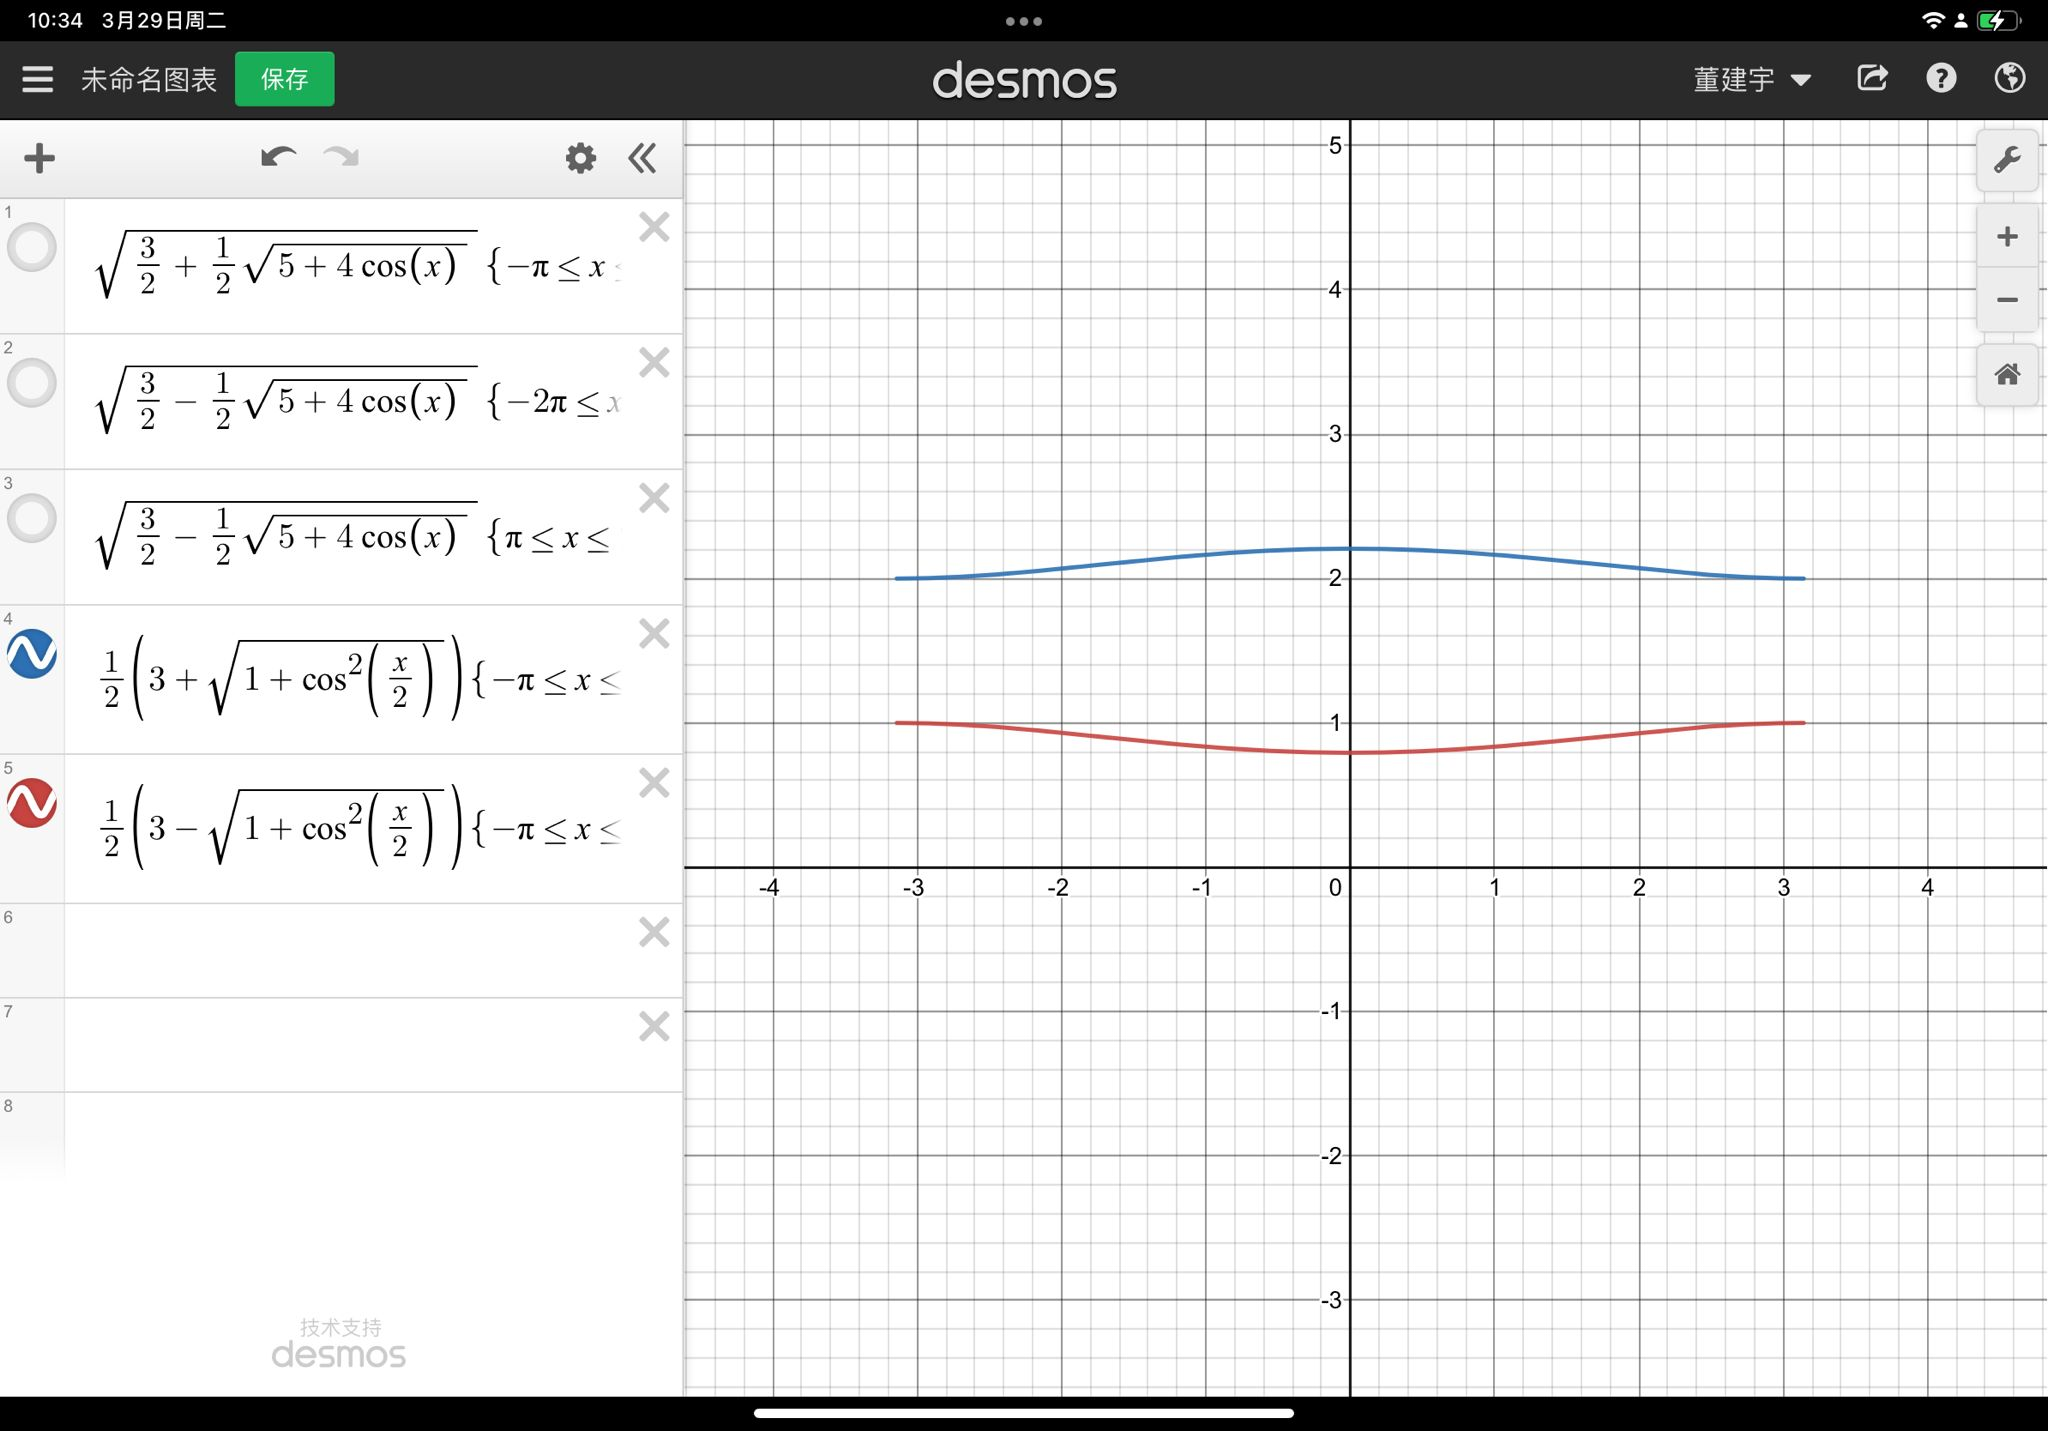
\includegraphics[scale=0.11]{reduced11.2.jpg}
\end{centering} \\
拓展布里渊区绘图如下:\\
\begin{centering}
	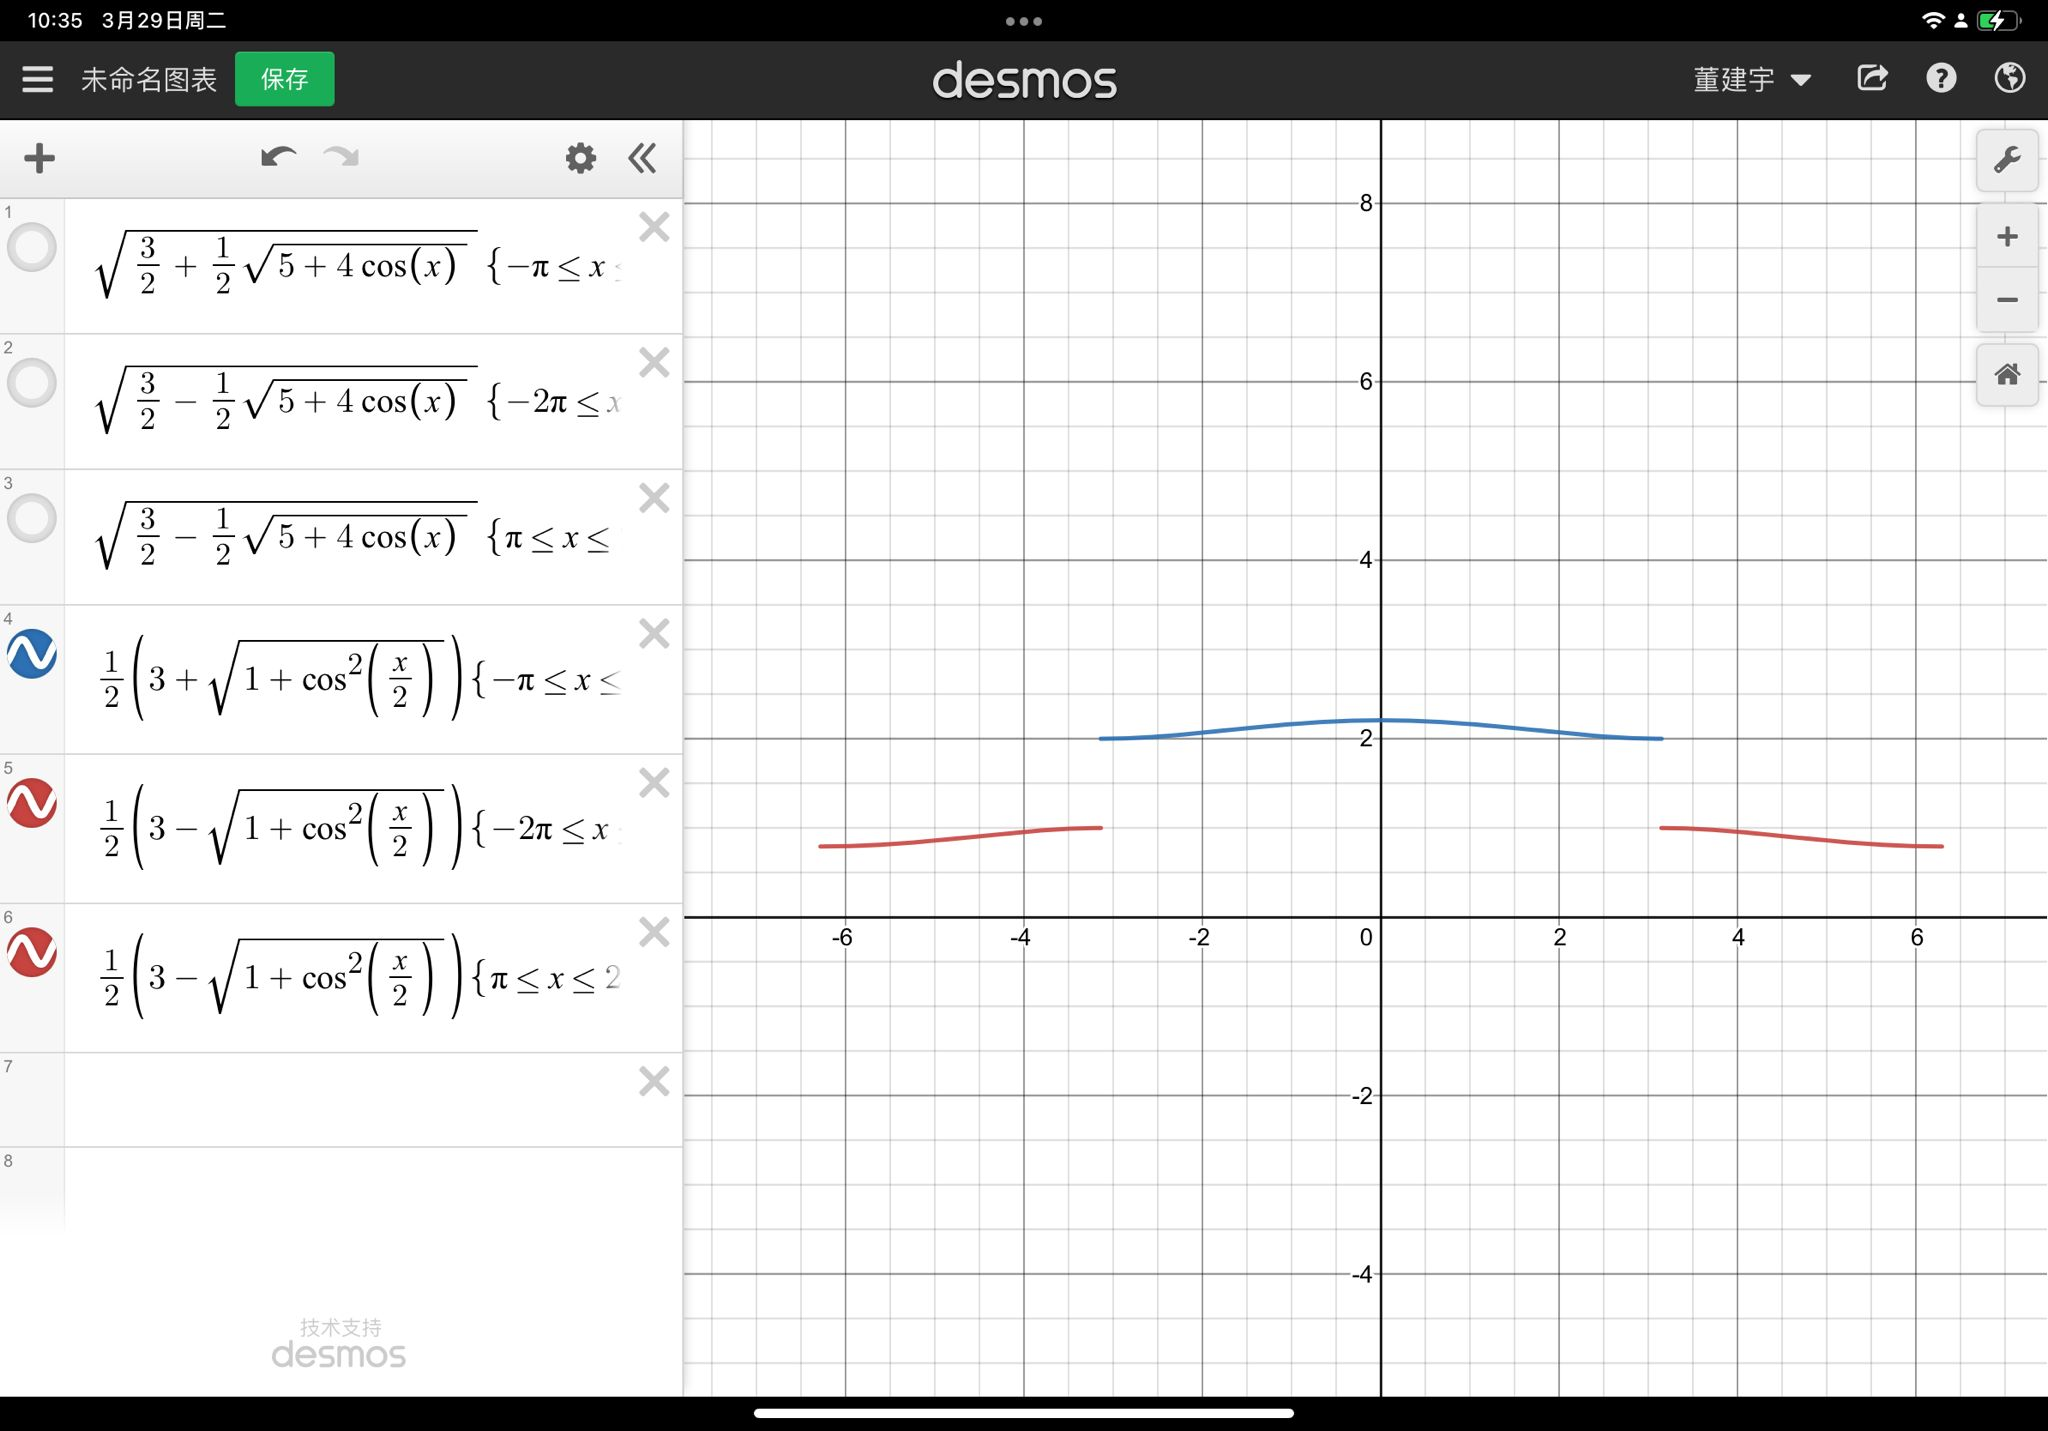
\includegraphics[scale=0.11]{extended11.2.jpg}
\end{centering} \\
$\triangleright$ 当$\epsilon_A = \epsilon_B = \epsilon$时,系统变为单原子链,有:
\[
	E_{\pm} = \epsilon \pm 2\vert t\cos(ka/2) \vert.
\]
$\triangleright$ 当$t$为无穷小量时,$E_+$与$E_-$将变得非常接近。 \\
$\triangleright$ 计算$\frac{dE_-}{dk}$得:
\[
	\frac{dE_-}{dk} = \frac{2at^2\sin(ka)}{\sqrt{(\epsilon_A-\epsilon_B)^2+16t^2\cos^2(ka/2)}}.
\]
在$k\to 0$的极限下,有:
\[
	\frac{dE_-}{dk} = \frac{2ka^2t^2}{\sqrt{(\epsilon_A-\epsilon_B)^2+16t^2}}.
\]
即有:
\[
	E_- = Constant + \frac{dE_-}{dk}k = Constant + \frac{2k^2a^2t^2}{\sqrt{(\epsilon_A-\epsilon_B)^2+16t^2}}.
\]
则有:
\[
	\frac{\hbar^2k^2}{2m^*} = \frac{2k^2a^2t^2}{\sqrt{(\epsilon_A-\epsilon_B)^2+16t^2}}.
\]
即有效质量为:
\[
	m^* = \frac{\hbar^2\sqrt{(\epsilon_A-\epsilon_B)^2+16t^2}}{4a^2t^2.}
\]
$\triangleright$ 如果每个原子都有一个价电子,那么每个元胞中恰好有两个价电子,恰好能填满能量较低的能级,如果$\epsilon_A = \epsilon_B$,则只要加电场就可以产生电流,即为导体;如果$\epsilon_A$与$\epsilon_B$相差不大,则可以消耗一部分能量用于激发,余下能量可以产生电流,即为半导体;如果$\epsilon_A$与$\epsilon_B$相差很大,则电子很难跃迁到高能级,即为绝缘体。 \\
$\triangleright$ 对于$LiF$,Li电负性很小,而F颠覆性很大,则有:
\[
	\epsilon_F >> \epsilon_{Li}.
\]
即LiF为绝缘体。
\end{tcolorbox}

\section{\textbf{(11.4)} \\
(a) Consider an atom with two orbitals, $A$ and $B$ having eigenenergies $\epsilon_{atomic}^A$ and $\epsilon_{atomic}^B$. Now suppose we make a one-dimensional chain of such atoms and let us assume that these orbitals remain orthogonal. We imagine hopping amplitudes $t_{AA}$ which allows an electron on orbital $A$ of a given atom to hop to orbital $A$ on the neighboring atom. Similarly we imagine a hopping amplitude $t_{BB}$ that allows an electron on orbital $B$ of a given atom to hop to orbital $B$ on the neighboring atom. (We assume that $V_0$, the energy shift of the atomic orbital due to neighboring atoms, is zero). \\
$\triangleright$ Calculate and sketch the dispersion of the two resulting bands. \\
$\triangleright$ If the atom is diatomic, derive a condition on the quantities $\epsilon_{atomic}^A - \epsilon_{atomic}^B$, as well as $t_{AA}$ and $t_{BB}$ which determines whether the system is a metal or an insulator. \\
(b) Now suppose that there is in addition a hopping term $t_{AB}$ which allows an electron in one atom in orbital $A$ to hop to orbital $B$ on the neighboring atom (and vice verse). What is the dispersion relation now?
}
\begin{tcolorbox}[breakable, colback = black!5!white, colframe = black]
\begin{enumerate}[(a)]
\item 由于态矢量仍满足正交关系,可分别对A,B列方程如下:
\[
	\begin{pmatrix}
		\epsilon_A & -t_{AA} & 0 & \cdots & -t_{AA} \\
		-t_{AA} & \epsilon_A & -t_{AA} & \cdots & 0 \\
		\vdots & \vdots & \vdots & & \vdots \\
		-t_{AA} & 0 & 0 & \cdots & \epsilon_A
	\end{pmatrix} \begin{pmatrix}
		a_1 \\
		a_2 \\
		\vdots \\
		a_N
	\end{pmatrix} = E_A\begin{pmatrix}
		a_1 \\
		a_2 \\
		\vdots \\
		a_N
	\end{pmatrix}
\]
\[
	\begin{pmatrix}
		\epsilon_B & -t_{BB} & 0 & \cdots & -t_{BB} \\
		-t_{BB} & \epsilon_B & -t_{BB} & \cdots & 0 \\
		\vdots & \vdots & \vdots & & \vdots \\
		-t_{BB} & 0 & 0 & \cdots & \epsilon_B
	\end{pmatrix} \begin{pmatrix}
		b_1 \\
		b_2 \\
		\vdots \\
		b_N
	\end{pmatrix} = E_B\begin{pmatrix}
		b_1 \\
		b_2 \\
		\vdots \\
		b_N
	\end{pmatrix}
\]
令$a_n = Ae^{ikna}$, $b_n = Be^{ikna}$,可以解得:
\[
	E_A = \epsilon_A - 2t_{AA}\cos(ka), ~~ E_B = \epsilon_B - 2t_{BB}\cos(ka).
\]
令$\epsilon_A = 1$, $\epsilon_B = 3$, $t_{AA} = 0.5$, $t_{BB} = 1$,则绘图如下: \\
\begin{centering}
	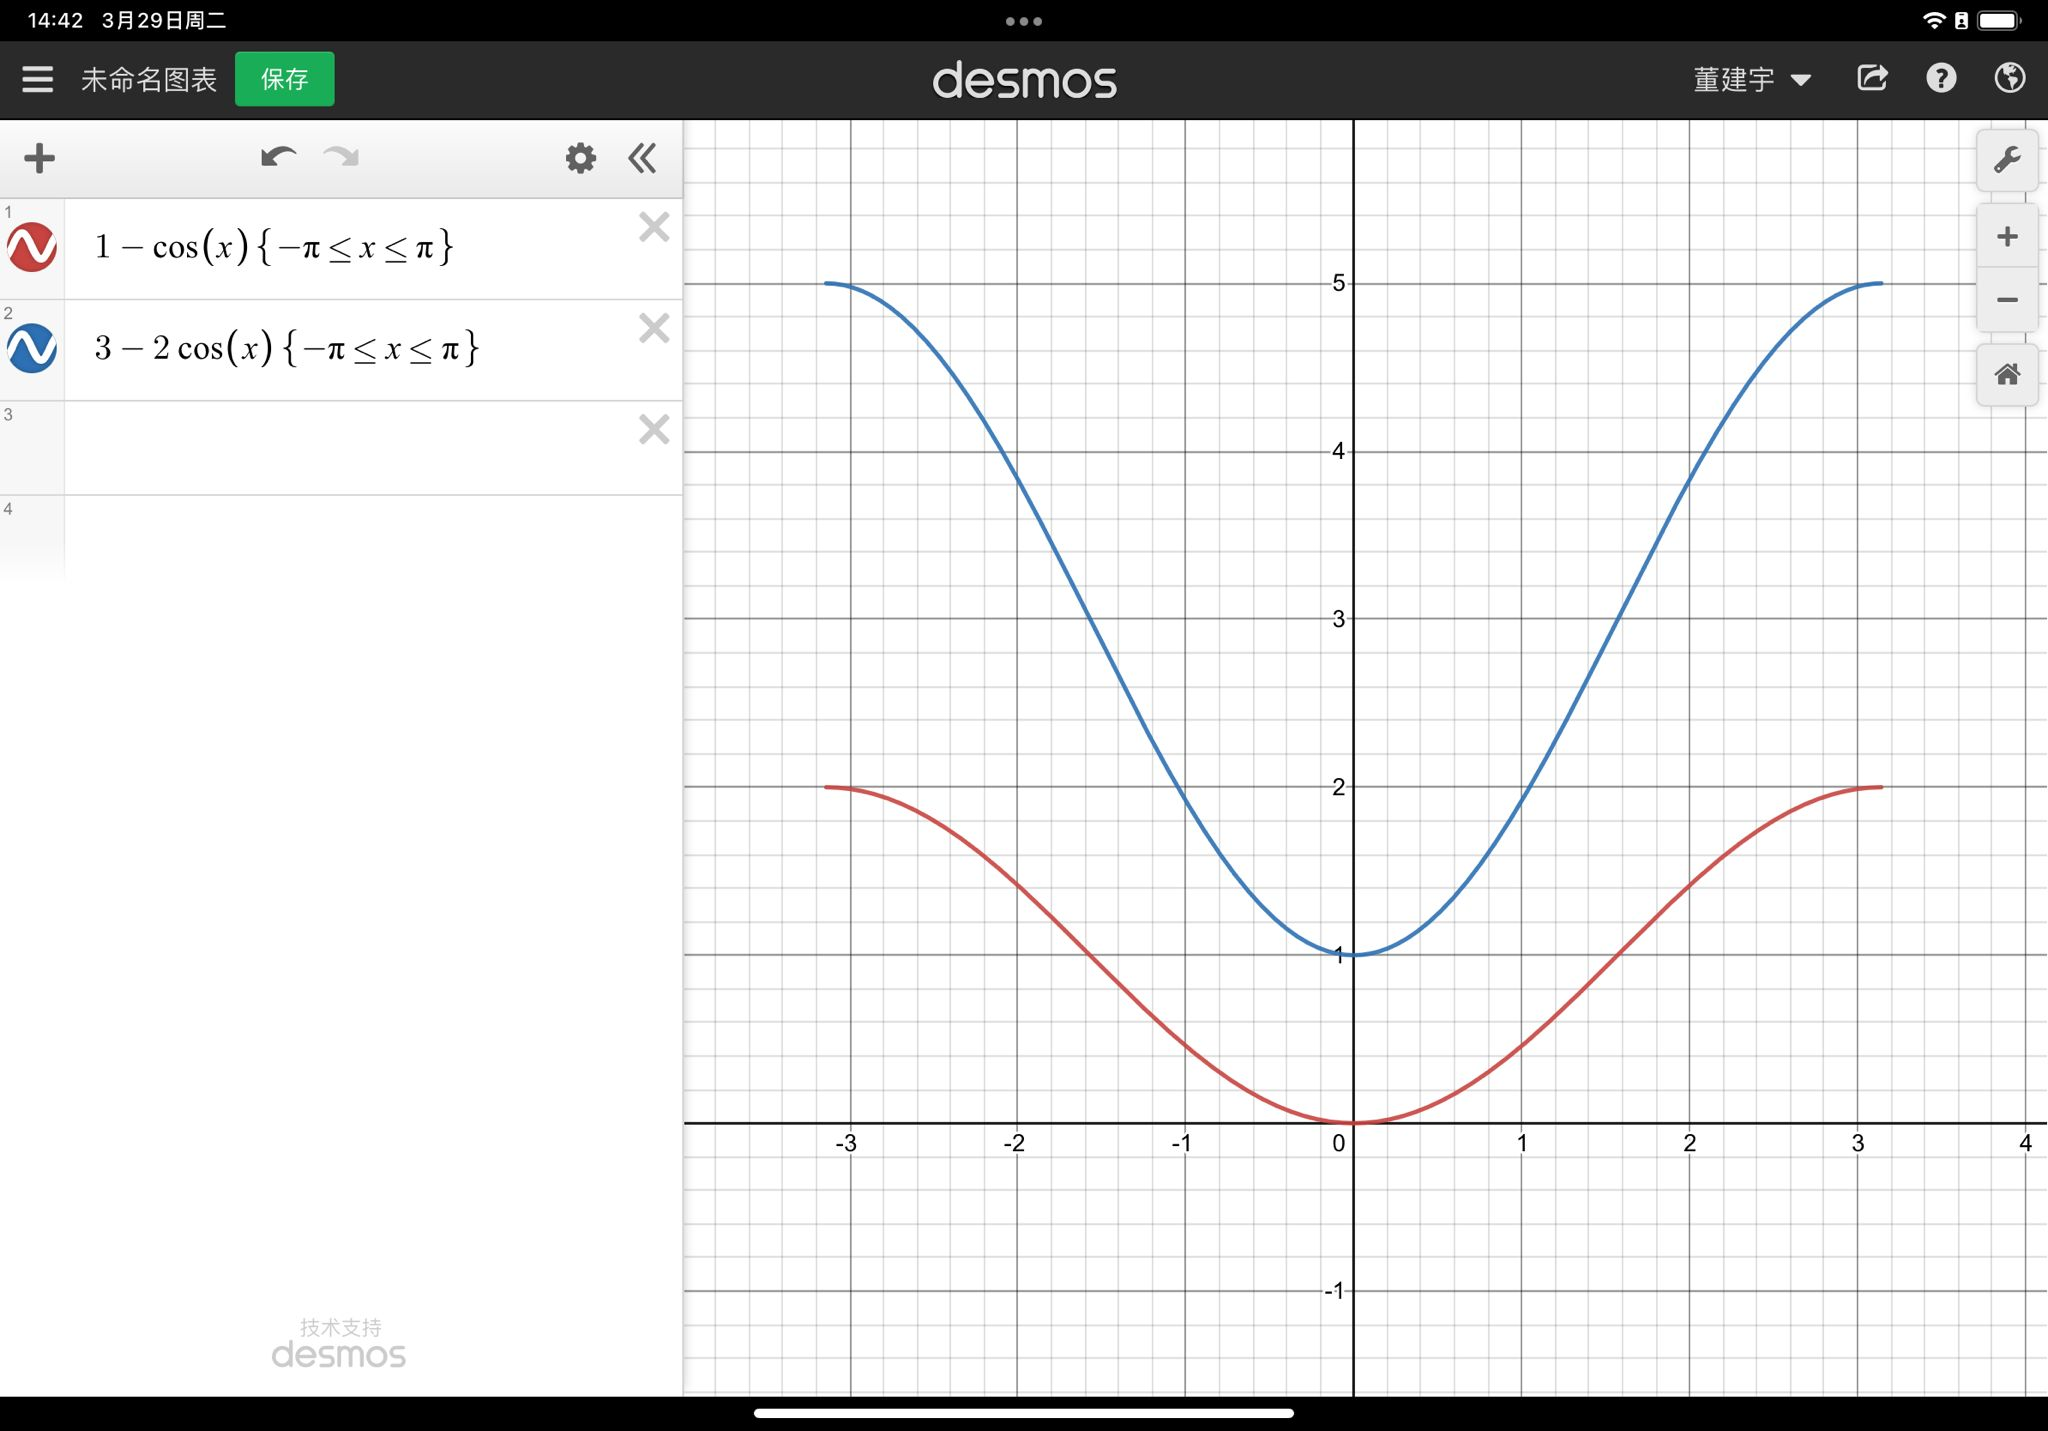
\includegraphics[scale = 0.11]{dispersion11.4.jpg}
\end{centering} \\
其中红线为$E_A$,蓝线为$E_B$。 \\
如果该体系为绝缘体,则$E_A$与$E_B$不存在交叠部分,即:
\[
	\epsilon_A - 2\vert t_{AA} \vert > \epsilon_B + 2\vert t_{BB} \vert
\]
或者
\[
	\epsilon_A + 2\vert t_{AA} \vert < \epsilon_B - 2\vert t_{BB} \vert
\]
否则,如果满足
\[
	\vert \epsilon_A - \epsilon_B \vert > 2(\vert t_{AA} \vert + \vert t_{BB} \vert)
\]
则体系为导体。 

\item 由题意可知,考虑第n个元胞中A、B原子,有:
\begin{align*}
	&-t_{AA}^* a_{n-1} - t_{AB}^* b_{n-1} + \epsilon_A a_n - t_{AA}a_{n+1} - t_{AB} b_{n+1} = Ea_n, \\
	&-t_{AB}^* a_{n-1} - t_{BB}^* b_{n-1} + \epsilon_B b_n - t_{AB}a_{n+1} - t_{BB} b_{n+1} = Eb_n.
\end{align*}
假设有:
\[
	a_n = A e^{ikna}, ~~ b_n = B e^{ikna},
\]
令
\begin{align*}
	&R_A = t_{AA}^*e^{-ika} + t_{AA}e^{ika} = 2\mathbf{Re}(t_{AA}e^{ika}) \\
	&R_B = t_{BB}^*e^{-ika} + t_{BB}e^{ika} = 2\mathbf{Re}(t_{BB}e^{ika}) \\
	&R_{AB} = t_{AB}^*e^{-ika} + t_{AB}e^{ika} = 2\mathbf{Re}(t_{AB}e^{ika})
\end{align*}
则有:
\begin{align*}
	&(E-\epsilon_A+T_{AA}) A + T_{AB} B = 0 \\
	&T_{AB} A + (E-\epsilon_B+T_{BB}) B = 0
\end{align*}
方程组存在非零解,有:
\[
	\left\vert \begin{matrix}
		E-\epsilon_A+T_{AA} & T_{AB} \\
		T_{AB} & E-\epsilon_B+T_{BB}
	\end{matrix} \right\vert = (E-\epsilon_A+T_{AA})(E-\epsilon_B+T_{BB}) - T_{AB}^2 = 0
\]
可以解得:
\[
	E_{\pm} = \frac{1}{2}(\epsilon_A+\epsilon_B-T_{AA}-T_{BB} \pm \sqrt{(\epsilon_A-T_{AA}-\epsilon_B+T_{BB})^2+4T_{AB}^2}).
\]
\end{enumerate}
\end{tcolorbox}


\section{\textbf{(11.5)} Electronic Impurity State \\
Consider the one-dimensional tight binding Hamiltonian given in Eq. 11.4. Now consider the situation where one of the atoms in the chain (atom $n=0$) is an impurity such that it has an atomic orbital energy which differs by $\Delta$ from all the other atomic orbital energies. In this case the Hamiltonian becomes 
\[
	H_{n,m} = \epsilon_0\delta_{n,m} - t(\delta_{n+1,m} + \delta_{n-1,m}) + \Delta \delta_{n,m}\delta_{n,0}.
\]
(a) Using an ansatz 
\[
	\phi_n = Ae^{-qa\vert n \vert}
\]
with $q$ real, and $a$ the lattice constant, show that there is a localized eigenstate for any negative $\Delta$, and find the eigenstate energy. This exercise is very similar to Exercise 9.6. \\
(b) Consider instead a continuum one-dimensional Hamiltonian with a delta-function potential 
\[
	H = -\frac{\hbar^2}{2m^*}\partial_x^2 + (a\Delta)\delta(x).
\]
Similarly show that there is a localized eigenstate for any negative $\Delta$ and find its energy. Compare your result to that of part (a).
}
\begin{tcolorbox}[breakable, colback = black!5!white, colframe = black]
\begin{enumerate}[(a)]
\item 当$n\neq 0$时,有:
\[
	E\phi_n = \epsilon_0\phi_n - t(\phi_{n-1}+\phi_{n+1}).
\]
带入
\[
	\phi_n = Ae^{-qa\vert n \vert}
\]
可得:
\[
	E = \epsilon_0 - t(e^{-qa}+e^{qa}).
\]
当$n = 0$时,有: 
\[
	E\phi_0 = (\epsilon_0+\Delta)\phi_0 - t(\phi_{-1}+\phi_1)
\]
则有:
\[
	E = \epsilon_0+\Delta - 2te^{-qa}.
\]
则可以解得:
\[
	\Delta = -2t\sinh(qa).
\]
则对于每一个负的$\Delta$,都有
\[
	qa = \sinh^{-1}(-\Delta/(2t)).
\]
即存在一个态,此态的能量为:
\[
	E_0 = \epsilon_0 - 2t\sqrt{1+\frac{\Delta^2}{4t^2}}.
\]

\item 假设仍有:
\[
	\psi(x) = Ae^{-px}
\]
则有:
\[
	-\frac{\hbar^2}{2m^*}\partial_x^2\psi(x) = -\frac{\hbar^2p^2}{2m^*}\psi(x)
\]
即
\[
	E = -\frac{\hbar^2p^2}{2m^*}.
\]
由于势能函数为$\delta$函数,满足连续性条件有:
\[
	\frac{\partial}{\partial x}\psi(0+) - \frac{\partial}{\partial x}\psi(0-) = -2p = \frac{2m^*a\Delta}{\hbar^2}.
\]
利用有效质量的表达式:
\[
	m^* = \frac{\hbar^2}{2a^2t}
\]
可得:
\[
	E_b = -\frac{\Delta^2}{4t}.
\]
注意到,(a)中当$\Delta \to 0$时,有:
\[
	E_a = \epsilon_0 - 2t\sqrt{1+\frac{\Delta^2}{4t^2}} \approx \epsilon_0 - 2t(1+\Delta^2/(8t^2)) = \epsilon_0 - 2t - \frac{\Delta^2}{4t}.
\]
选取合适的基态能量满足:$\epsilon_0 - 2t = 0$,则有:
\[
	E_a = -\frac{\Delta^2}{4t} = E_b.
\]
\end{enumerate}
\end{tcolorbox}
\end{document}